%!TEX root = ../dokumentation.tex

\chapter{Datenbankverbindung}
\label{ch:Datenbankverbindung}
Die db.js legt die Verbindung zur Datenbank fest. Hier wird der URL-Pfad zum Mongo-Datenbank-Container festgelegt und exportiert. Somit kann diese URL von den anderen Teilen der Anwendung aufgerufen werden.

\begin{figure}[h]
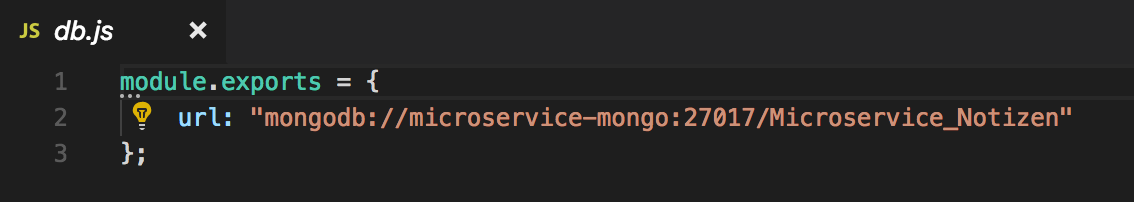
\includegraphics[height=.18\textwidth]{Datenbankconnection.png}
\vspace{3pt}
\caption{Schaubild\footnotemark}
\label{fig:blueant}
\end{figure}

Zu beachten ist hier, dass der Pfad zum selbst bezeichneten Container festgelegt wird, nicht zu einer absoluten IP oder dem Localhost. \glqq  microservice-mongo\grqq{} beschreibt den Mongo-Db-Container der in der docker-compose.yaml erstellt wurde. \glqq  :27017\grqq{} ist hierbei der virtuelle Port der vom microservice-mongo-Container bereitgestellt wird. \glqq  Microservice\_Notizen\grqq{} ist in diesem Fall die konkrete Datenbank innerhalb der Mongo-DB.


